\documentclass[../main.tex]{subfiles}
\begin{document}

\section{Empirical Evidence}
\label{sec:application}

The empirical analysis examines the magnitude and structure of target-coefficient sensitivity across ten published studies built around randomized experimental variation. One prespecified target estimand from each study is evaluated under a common deletion protocol. The cross-study analysis measures how far each coefficient can move within a small deletion budget, while selected applications examine how influential-set membership persists, changes with \(k\), or concentrates across observable groups. Each result is conditional on the validated audit specification and realised estimation sample. Study-specific specifications, validation checks, and implementation details are reported in \autoref{app:application-details}.

\subsection{Audit Design}
\label{subsec:application-design}

Each empirical audit preserves the validated specification associated with its selected estimand while applying a common deletion protocol. The relevant estimation sample is first reproduced and the baseline target coefficient is verified. Candidate deletion sets are then constructed in both directions of coefficient movement over deletion sizes up to approximately \(5\%\) of the estimation sample. The search uses the fixed-residualised MIS objective, after which each selected set undergoes \emph{full-refit validation} using the estimator associated with the frozen audit specification. The resulting sensitivity paths therefore record coefficient movement after re-estimation on the retained sample.

The common search requires an MIS-compatible linear representation of the target coefficient. Fixed effects, fixed weights, and nuisance specifications are retained only after baseline equivalence has been verified. When the headline estimator lies outside the current linear search framework, the audit uses a documented linear companion or robustness specification. \autoref{app:application-details} records the resulting estimand and specification for each study.

The empirical analysis targets finite-sample point-estimate sensitivity within each validated specification. Randomized assignment supplies the identifying variation in the source studies, while the deletion analysis measures dependence of the audited coefficient on its realised estimation sample. These are separate inferential objects. An experimentally identified effect can therefore exhibit substantial finite-sample coefficient sensitivity within a particular audited specification.

\subsection{Magnitude of Target-Coefficient Sensitivity}
\label{subsec:application-sensitivity}

The ten audited coefficients differ substantially in how quickly they move under small deletion budgets. To compare this sensitivity across studies, the audit records the first searched deletion fraction at which the full-refit coefficient reaches a prespecified threshold relative to its full-sample value. The thresholds are a \(50\%\) attenuation, a \(50\%\) amplification, and a zero crossing. Each threshold is evaluated within a deletion budget of approximately \(5\%\) of the corresponding estimation sample.

\begin{figure}[htbp]
	\centering
	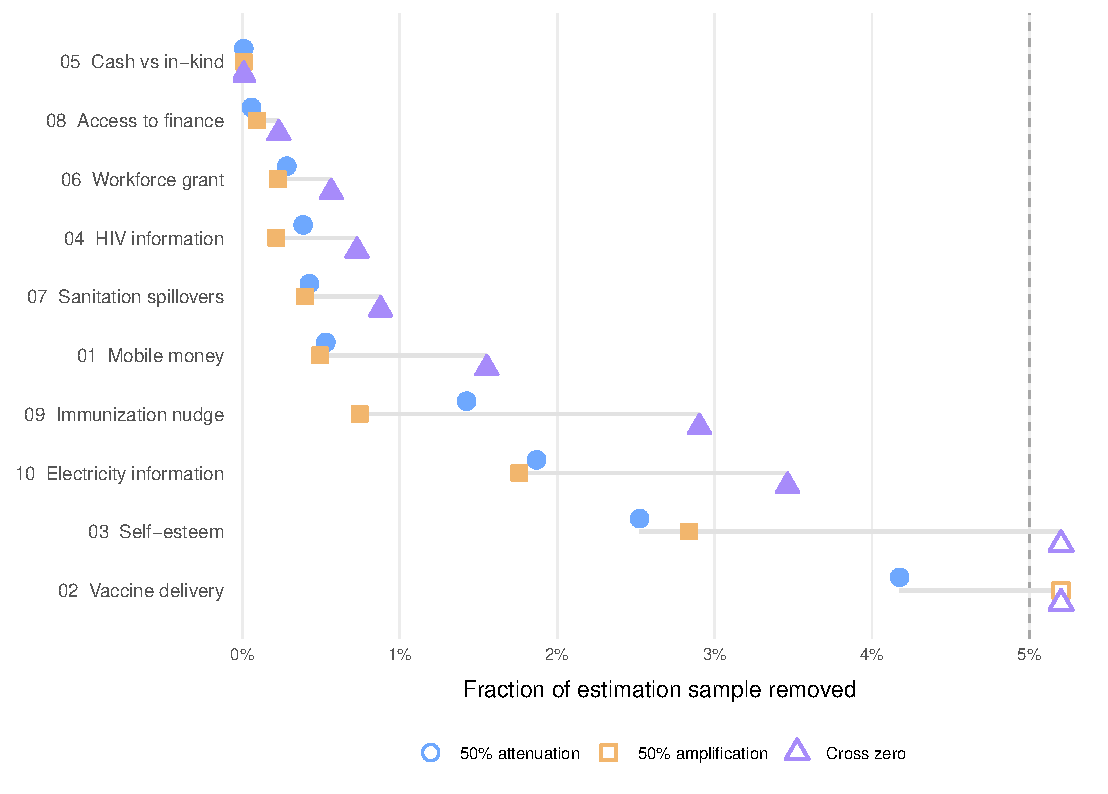
\includegraphics[width=\linewidth]{../../application/00_cross_study/figures/main/05_fig1_sensitivity_thresholds.pdf}
	\caption{Cross-study target-coefficient sensitivity thresholds for the ten selected estimands. Markers report the first searched deletion fraction at which the refitted audited coefficient reaches a \(50\%\) attenuation, a \(50\%\) amplification, or a zero crossing. Hollow markers indicate that the corresponding threshold is not reached within the prespecified deletion budget of approximately \(5\%\) of the estimation sample.}
	\label{fig:application-sensitivity-thresholds}
\end{figure}

\begin{table}[htbp]
\centering
\caption{Cross-study target-coefficient sensitivity thresholds.}
\label{tab:application-sensitivity}
\small
\resizebox{\textwidth}{!}{%
\begin{tabular}{lrrrrr}
\toprule
Study & $N$ & $\widehat{\beta}_{\mathrm{full}}$ & 50\% attenuation & 50\% amplification & Cross zero \\
\midrule
01  Mobile money & 2,639 & 69.21 & 0.53\% (14) & 0.49\% (13) & 1.55\% (41) \\
02  Vaccine delivery & 12,096 & 0.2935 & 4.17\% (505) & Not reached & Not reached \\
03  Self-esteem & 634 & 0.2317 & 2.52\% (16) & 2.84\% (18) & Not reached \\
04  HIV information & 2,332 & -0.1566 & 0.39\% (9) & 0.21\% (5) & 0.73\% (17) \\
05  Cash vs in-kind & 10,985 & -0.8861 & 0.009\% (1) & 0.009\% (1) & 0.009\% (1) \\
06  Workforce grant & 1,770 & 0.0231 & 0.28\% (5) & 0.23\% (4) & 0.56\% (10) \\
07  Sanitation spillovers & 3,757 & -0.00976 & 0.43\% (16) & 0.40\% (15) & 0.88\% (33) \\
08  Access to finance & 8,612 & -0.0855 & 0.058\% (5) & 0.093\% (8) & 0.23\% (20) \\
09  Immunization nudge & 7,370 & 0.00402 & 1.42\% (105) & 0.75\% (55) & 2.90\% (214) \\
10  Electricity information & 1,819 & -0.1168 & 1.87\% (34) & 1.76\% (32) & 3.46\% (63) \\
\bottomrule
\end{tabular}%
}
\begin{minipage}{0.98\textwidth}
\footnotesize
\textit{Notes:} Threshold entries report the fraction of the estimation sample removed, with the corresponding number of deleted observations in parentheses. The normalized coefficient is $R_k=\widehat{\beta}_{-S_k}/\widehat{\beta}_{\mathrm{full}}$. A 50\% attenuation is first reached when $R_k\leq0.5$; a 50\% amplification is first reached when $R_k\geq1.5$; and the coefficient crosses zero when $R_k\leq0$. ``Not reached'' indicates that the threshold is not attained within the study's prespecified deletion budget of at most approximately 5\% of the estimation sample.
\end{minipage}
\end{table}


Eight of the ten audited coefficients cross zero along at least one searched deletion path within the prespecified budget (\autoref{fig:application-sensitivity-thresholds} and \autoref{tab:application-sensitivity}). The first zero crossing ranges from a single deleted observation, approximately \(0.009\%\) of the estimation sample in the cash-versus-in-kind application, to \(63\) observations, approximately \(3.46\%\), in the electricity-information application. The required deletion fraction therefore varies markedly across the audited estimands. This variation characterises substantial cross-study heterogeneity in the magnitude of finite-sample target-coefficient sensitivity.

The vaccine-delivery and self-esteem applications exhibit sensitivity without a sign reversal within the searched range. The vaccine-delivery estimate reaches a \(50\%\) attenuation at approximately \(4.17\%\) deletion, while the self-esteem coefficient also shows material movement within the audit budget. Sign reversal therefore captures one dimension of coefficient sensitivity. Attenuation and amplification provide additional evidence about the magnitude of dependence on selected subsets.

\subsection{Structure of Influential Sets}
\label{subsec:application-interpretation}

Influential sets also differ in their composition as the deletion budget changes and across application contexts. The access-to-finance and health-information audits show contrasting patterns of persistence across values of \(k\), while the immunization audit provides evidence of geographic concentration. These patterns complement the cross-study sensitivity thresholds by characterising the structure of the observations carrying target-coefficient influence.

\begin{figure}[htbp]
	\centering
	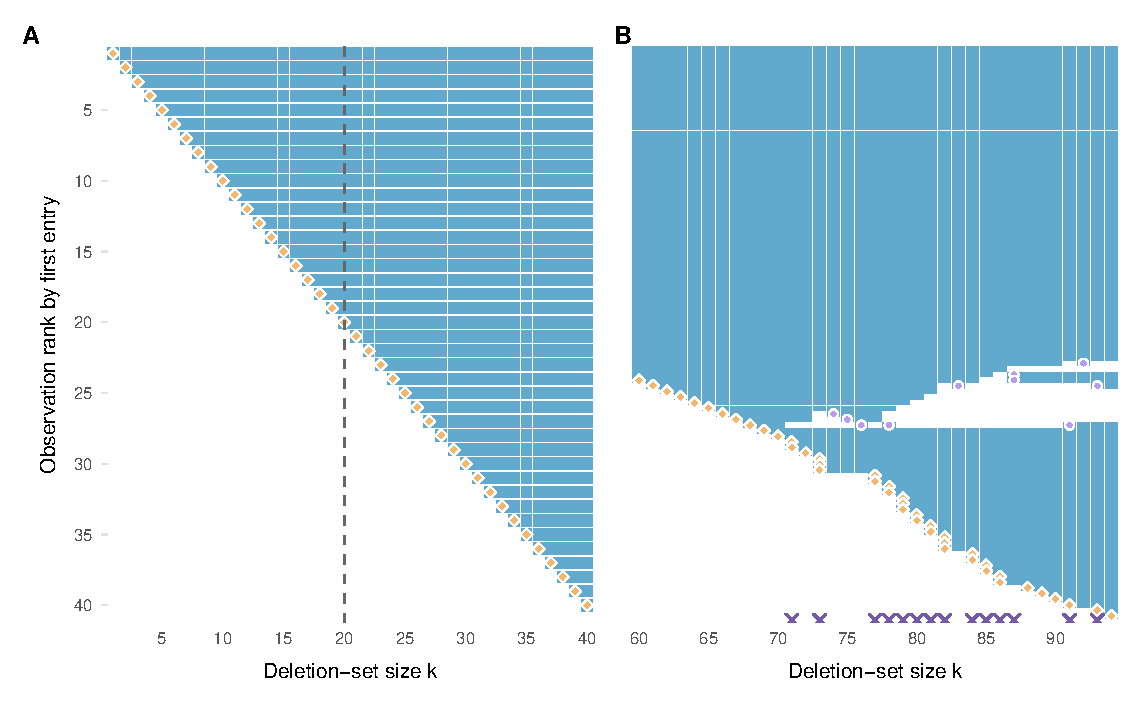
\includegraphics[width=\linewidth]{../../application/00_cross_study/figures/main/05_fig2_influential_set_persistence.pdf}
	\caption{Influential-set persistence in two empirical applications. Panel A reports the access-to-finance application of \textcite{cai2024indirect}, where influential observations accumulate through a nested path over the displayed deletion range. Panel B reports the health-information application of \textcite{ciancio2025surviving}, where influential-set membership changes over the displayed deletion range. The dashed line marks the first zero crossing along the displayed directional path.}
	\label{fig:application-persistence}
\end{figure}

The access-to-finance audit combines strong coefficient sensitivity with a persistent influential core. \textcite{cai2024indirect} study direct and competitor-exposure effects of experimentally induced access to finance, and the audit targets the competitor-treatment exposure coefficient for firm log sales. Its validated full-sample estimate is \(-0.0855\), and the coefficient first crosses zero after deleting \(20\) of \(8{,}612\) observations, approximately \(0.23\%\) of the estimation sample. As the deletion budget increases, observations entering at smaller values of \(k\) tend to remain in the selected set (\autoref{fig:application-persistence}). The sensitivity path therefore contains a relatively stable influential core.

The health-information audit shows a different structure despite a similarly small sign-reversing deletion set. \textcite{ciancio2025surviving} study the consequences of learning an HIV-positive diagnosis, and the present audit considers their reported OLS companion specification for survival. The validated full-sample coefficient is \(-0.1566\), and it first crosses zero after deleting \(17\) of \(2{,}332\) observations, approximately \(0.73\%\) of the estimation sample. Influential-set membership changes repeatedly as \(k\) increases, producing a non-nested sensitivity path (\autoref{fig:application-persistence}). The source study's preferred IV/GMM causal specification lies outside the current linear MIS audit.

The contrast shows that similar sensitivity magnitudes can arise from different influential-set structures. One coefficient depends on a relatively persistent core, while the other is supported by sets whose membership changes across deletion budgets. Target-coefficient sensitivity therefore has a compositional dimension in addition to the magnitude of coefficient movement.

The immunization audit provides a third structural pattern through geographic concentration. \textcite{banerjee2025selecting} evaluate randomized combinations of immunization reminders, incentives, and community ambassadors in Haryana, India. The audit targets the pooled policy coefficient for immunizations per dollar associated with the selected policy specification. Its validated full-sample estimate is \(0.0040\), and the coefficient first crosses zero after deleting \(214\) of \(7{,}370\) village-month observations, approximately \(2.90\%\) of the estimation sample.

\begin{figure}[htbp]
	\centering
	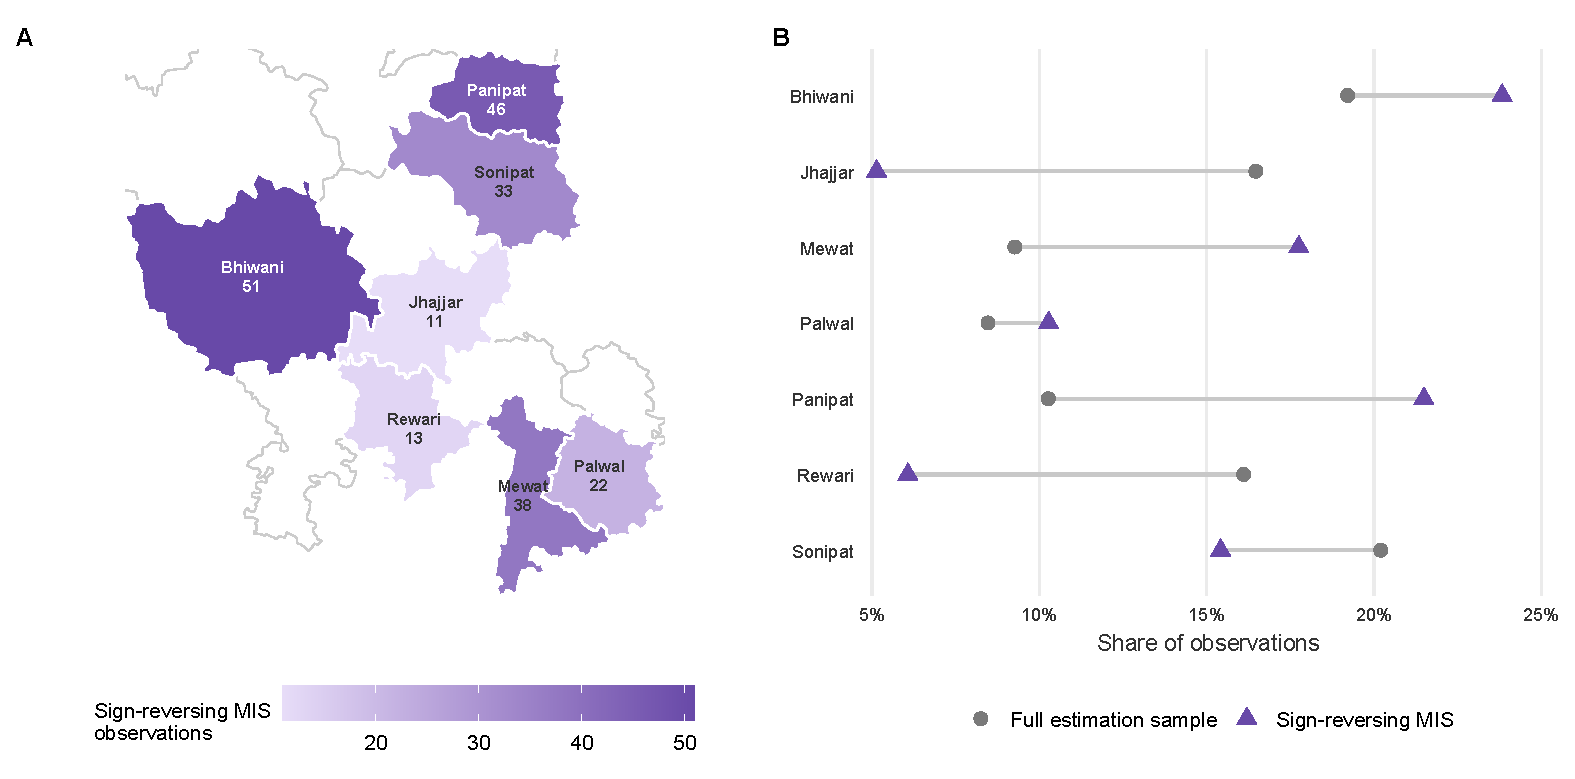
\includegraphics[width=\linewidth]{../../application/09_StMEN/fig_spatial_concentration.pdf}
	\caption{Spatial composition of the first sign-reversing MIS in the immunization application of \textcite{banerjee2025selecting}. Panel A reports the number of sign-reversing MIS observations in each of the seven study districts. Panel B compares each district's share of the full estimation sample with its share of the \(214\)-observation sign-reversing MIS. District boundaries follow the Census 2011 definitions retained in the study data.}
	\label{fig:application-spatial-concentration}
\end{figure}

The first sign-reversing set is unevenly distributed across the seven study districts (\autoref{fig:application-spatial-concentration}). Panipat and Mewat contribute larger shares of the selected set than of the full estimation sample, while Jhajjar and Rewari contribute smaller shares. The observations carrying coefficient influence therefore have an observable geographic structure in this application. This concentration describes the composition of the selected set without identifying the mechanism that generates its influence.

The empirical audits reveal heterogeneity in both the magnitude and structure of finite-sample target-coefficient sensitivity. Across the ten selected estimands, threshold crossings occur at substantially different deletion fractions. The selected sets also differ in persistence and observable composition, ranging from relatively stable influential cores to non-nested paths and geographically concentrated subsets. These patterns characterise how audited coefficients depend on particular parts of their realised estimation samples.

The empirical evidence characterises finite-sample sensitivity of the selected estimands within their validated audit specifications and stated deletion budgets. The source studies' identification strategies and other estimands remain separate objects of analysis. Study-specific specifications, validation checks, and scope qualifications are reported in \autoref{app:application-details}. Together with the simulation evidence, these audits show that target-coefficient sensitivity varies in both magnitude and structure across mechanisms and realised empirical samples.

\end{document}
